\documentclass{article}

%Deutsche Sprachunterstützung
\usepackage[utf8]{inputenc}
\usepackage[ngerman]{babel}
\usepackage{marvosym}
\DeclareUnicodeCharacter{20AC}{\EUR}

%Für das Einbinden von Bildern
%\usepackage{graphicx}

%Tabellen
\usepackage{array}

%Tabellen automatisch schoener
\usepackage{booktabs}

%Caption
\usepackage{caption}
\usepackage{subcaption}

%Formeln
\usepackage{mathtools}
\usepackage{amsmath}
\usepackage{amssymb}
\usepackage{amstext}
\usepackage{dsfont}

%\usepackage{mnsymbol}

%Vectorpfeile schöner
\usepackage{esvect}

%Formatierung
\usepackage[T1]{fontenc}
\usepackage{lmodern}
\usepackage{microtype}
%\usepackage[german=guillemets]{csquotes}

%Formatierungsanweisungen
\newcommand{\wichtig}[1]{\underline{\large{#1}}}
\newcommand{\aref}[1]{(s.Abb. \ref{#1})}
\newcommand{\R}{\mathbb{R}}
\newcommand{\K}{\mathbb{K}}
\newcommand{\C}{\mathbb{C}}
\begin{document}
\section{Aufgabe 3}
Gegebene Schaltung:\\
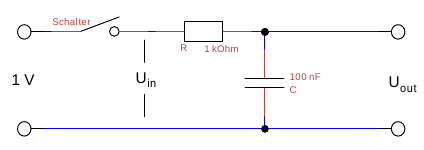
\includegraphics[width=\textwidth]{../daten/Messdaten/plots/schalt_tief2}
Gemessene3 Sprungreaktion:\\
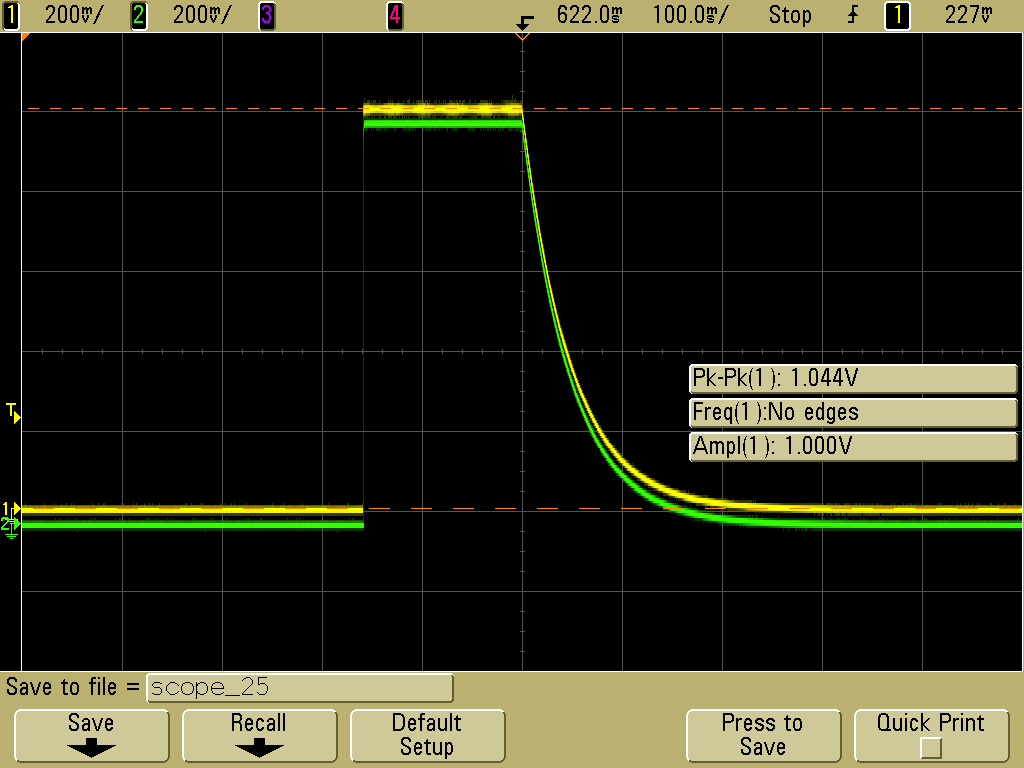
\includegraphics[width=\textwidth]{../daten/scope_25}

Gesucht: Zeitkonstante $\tau = R \cdot C$\\
Sprungreaktion ist in diesem Fall der Entladevorgang des Kondensators, gegeben durch:
\begin{equation}
U(t) = U_0 * \exp(-\frac{t}{\tau}),  \tau = \frac{1}{R\cdot C}
\end{equation}
Strategie: Setze $t=\tau$ $\Rightarrow  U(\tau) = U_0 \cdot \exp(-1)$
und suche den Wert $\frac{U(t)}{U_0} = \frac{1}{e}$ in der Messtabelle:
\begin{equation}
t \approx 0.045 s
\end{equation}
Errechneter Wert:
\begin{equation}
\tau = R \cdot C = 10^{-7} \cdot 10^{3} = 10^{-4}
\end{equation}
\end{document}